\begin{figure}[t!]
  \vspace{-3mm}
  \centering
  \begin{minipage}[c]{0.47\textwidth}
    \centering
    \begin{adjustbox}{width=\textwidth}
    \begin{tabular}{lccc}
    \toprule
    \textbf{Statistic} & \textbf{Number} & \textbf{Bnd.} & \textbf{Rel.} \\
    \midrule
    Theorem categories & 29 & - & - \\
    Named theorems & 83 & - & - \\
    \midrule
    Training problems (for training) & 1252 & 626 & 626 \\
    - With theorem annotations & 962 & 482 & 480 \\
    - With solution annotations & 1252 & 626 & 626 \\
    - Avg. solutions per problem & 1.05 & 1.06 & 1.05 \\
    - Max solutions per problem & 4 & 4 & 4 \\
    \midrule
    Dev problems (for development) & 100 & 50 & 50 \\
    Test problems (for benchmarking) & 200 & 96 & 104 \\
    \bottomrule
    \end{tabular}
    \end{adjustbox}
    \captionof{table}{Statistics of the \dataset dataset.}
    \label{tab:data_statistics}
  \end{minipage}
  \hfill
  \begin{minipage}[c]{0.50\textwidth}
    \centering
    % \vspace{-1mm}
    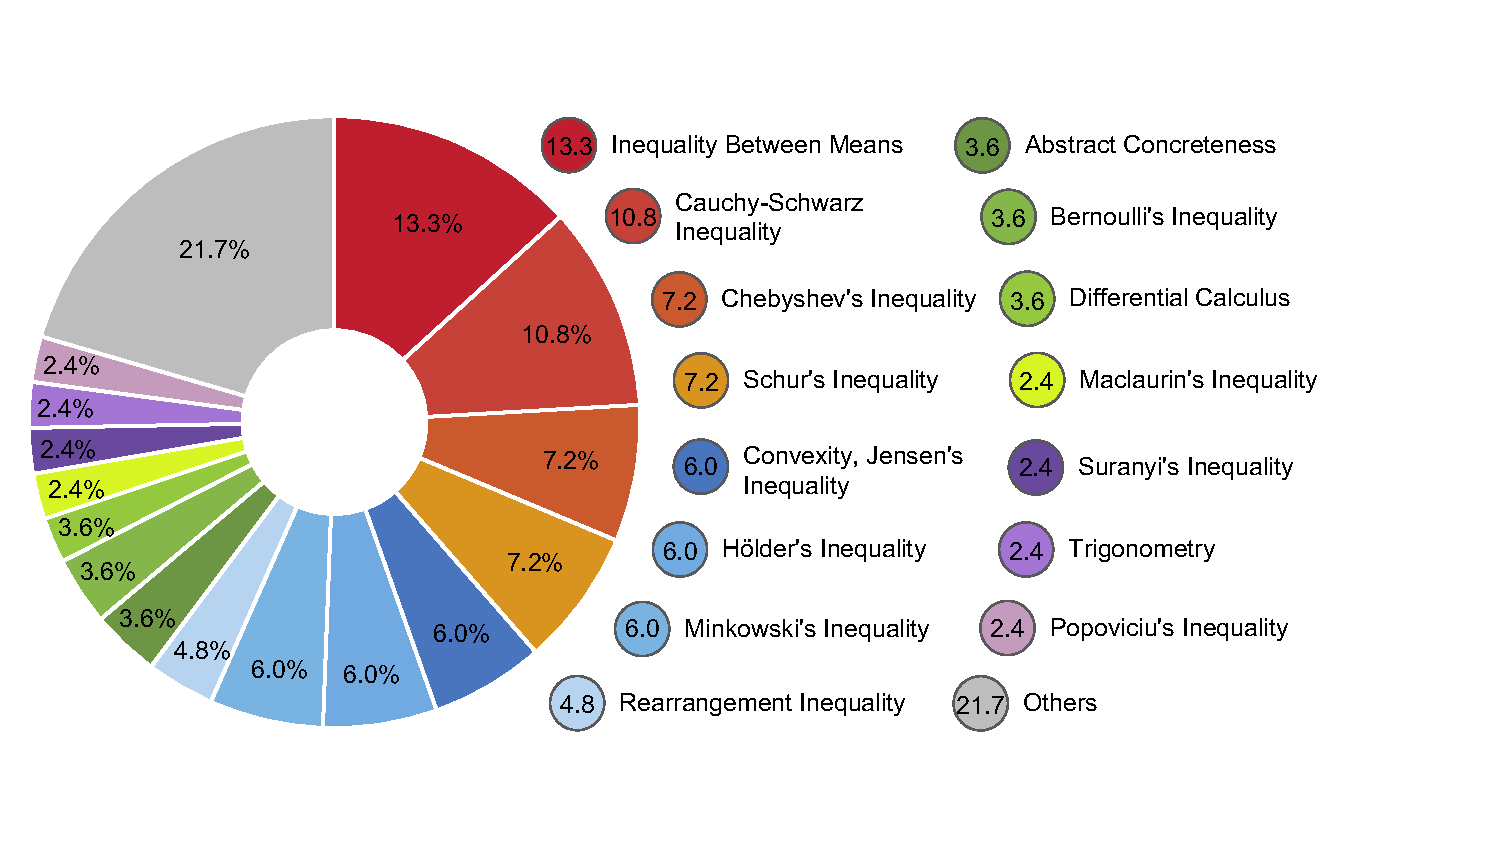
\includegraphics[width=1.0\linewidth]{figs/theorem_category_pie_chart.pdf}
    \vspace{-4mm}
    \captionof{figure}{Distribution of theorem categories.}
    \label{fig:theorem_category_pie}
  \end{minipage}
  \vspace{-7mm}
\end{figure}